\documentclass[aps,prl,twocolumn,showpacs,superscriptaddress,groupedaddress,10pt]{revtex4-1}  % for review and submission
%\documentclass[aps,twocolumn,floatfix,prl,10pt]{revtex4-1}
%\documentclass[letterpaper,10pt,prl,twocolumn,aps]{revtex4-1}
%\documentclass[aps,preprint,floatfix,prl]{revtex4-1}
%\usepackage{fullpage}
\usepackage{amsmath}
\usepackage{amsfonts}
\usepackage{amssymb}
\usepackage{graphicx}
%\usepackage{slashbox}
\usepackage{color}
\usepackage{longtable}
\usepackage{array}
\usepackage{dashrule}
\usepackage{dcolumn}% Align table columns on decimal point
%\usepackage{dcolumn}% Align table columns on decimal point
\usepackage{bm}% bold math
\usepackage{ifthen}
\usepackage{amsthm} % Theorem Formatting
\usepackage{amssymb}	% Math symbols such as \mathbb
\usepackage{calrsfs}
\usepackage{subfigure}
\graphicspath{ {images/}{images/Growth_Rate_Cont_Plots/} }
\newcommand{\ellcap}{{\ell_\text{c}}}
\newcommand{\Fh}{{\boldsymbol{F}_h}}
\newcommand{\Fv}{{\boldsymbol{F}_v}}
\newcommand{\Tv}{{\boldsymbol{T}}}
\newcommand{\bn}{{\boldsymbol{n}}}
\newcommand{\bt}{{\boldsymbol{t}}}
\newcommand{\bz}{{\boldsymbol{z}}}
\newcommand{\bx}{{\boldsymbol{x}}}
\newcommand{\by}{{\boldsymbol{y}}}
\newcommand{\bT}{{\boldsymbol{T}}}
\newcommand{\bu}{\mathbf{u}}
\newcommand{\grad}{\mathbf{\nabla}}
\newcommand{\del}{\partial}

\newcommand{\shreyas}[1]{{\bf (#1)}}

\begin{document}
\title{Waving and swaying}
\author{Ravi Singh}
\affiliation{Brown University, Providence RI 02912 USA}
\author{L. Mahadevan}
\affiliation{Harvard University, Cambridge MA 02138 USA}
\author{Mahesh Bandi\footnote{work performed while visiting Brown University}}
\affiliation{Okinawa Institute of Science and Technology, Okinawa, Japan}
\author{Amala Mahadevan}
\affiliation{Woods Hold Institute of Oceanography, Woods Hole MA USA}
\author{Shreyas Mandre}
\affiliation{Brown University, Providence RI 02912 USA}

\begin{abstract}
%The spontaneous waving of marine grass is thought to be due to a Kelvin-Helmholtz instability resulting from an inflection point in the flow profile. 
%We find that this inflection point is located inside the grass canopy but it does not lead to Kelvin Helmholtz instability which is 
%normally observed in a free shear layer. We also show that the wavelength of coherent vortices scales with the unvegetated water depth, and not with 
%the shear layer thickness as predicted by a theory based on Kelvin-Helmholtz instability. Based on these results, we propose a mechanism for waving 
%marine grass based on the shear instability of the flow above the canopy.

%The spontaneous waving of marine grass is though to be due to a Kelving-helmholtz instability resulting from strong shear near top of grass. On the contrary
%we find that strong velocity shear resulting from vertical discontinuity of drag due to presence of grass does not lead to Kelvin-Helmholtz instability which is 
%normally observed in free shear flows. We also show that wavelength of coherent vortices scales with the unvegetated water depth. Based on these results, 
%we propose an alternative mechanism which attributes waving of marine grass on shear instability of flow above the canopy. 

The spontaneous waving of marine grass is thought to be due to a Kelvin-Helmholtz instability resulting from an inflection point in the flow profile. We find that this inflection point
is located near the tip of grass canopy. Our analysis shows that flow in presence of grass become unstable not only through a mechanism of Kelvin-Helmholtz instability associated with 
inflection point but also through shear instability of flow above grass coupled with the porous flow through grass bed.
\end{abstract}
\maketitle

%\section{Introduction}
Sea grasses exhibit rich set of dynamics due to their interaction with the flow of water and can considerably affect surrounding hydrodynamic conditions.
Resulting changes in hydrodynamic conditions can influence number of environmental variables and processes such as 
transport of sediments, contaminants, dissolved oxygen, plant growth and biomass production etc \cite{Fonseca87,Nepf99}. 
The response of flexible grass canopies to steady current in form of large amplitude coherent oscillation, known as mo-nami \cite{AckermanOkubo93}, plays a central role
in the recruitment of microscopic marine organism such as blue mussel larvae \cite{Grizzle96}. The hydrodynamic mechanism underlying monami is the focus of this paper. 
\newline
Similar phenomenon of large amplitude coherent oscillation of canopy in atmospheric flow known as ho-nami\cite{Inoue56,Raupach96}, have also been observed.
A crucial difference between the atmospheric and aquatic flow is that the atmospheric flows are essentially unbounded vertically. Another major
difference between the two is the considerable difference of stiffness of canopies; terrestrial canopies tend to be much more rigid than aquatic canopies.
Due to these differences between aquatic and marine flow, our analysis of flow in presence of flexible grass in a bounded domian is applicable only to marine canopies. 
\newline   
Existing explanation of mo-nami invokes the existence of strong shear near the top of the canopy \cite{Ghisal02,Raupach96} due to
different amounts of drag experienced by fluid in and above the canopy. This shear layer is assumed to become unstable to coherent vortices through a mechanism similar to 
Kelvin-Helmholtz instability. Influence of these coherent eddies over sea grasses is manifested in their large amplitude synchronous oscillations.
%Sea grasses exhibit large amplitude wave like motion in response to these eddies propagating downstream.
%are exhibited in form of large amplitude oscillations knows as mo-nami.
\newline
While shear layer model successfully appears to predict frequency of mo-nami for number of experimental observations,
several aspect of existing theory remain unsatisfactory. First, linear stability analysis of base flow does not take into account influence of drag due to grass hence not a self 
consistent theory. Second, classical free shear flow is known to be unstable above a very small Reynolds number $\leq 10 $, whereas observed critical 
Reynolds number\cite{Grizzle96} (Grizzle 1996) for monami is much higher $\approx O(1000)$. Finally, the thickness of the free shear layer, defined as the momentum thickness of the boundary layer near the grass tip, is in many cases comparable to the unvegetated layer thickness, and therefore inconsistent with the assumptions of the free shear layer instability. These drawbacks of existing theory suggest that flow through vegetation requires further investigation for better understanding of phenomenon.

In this paper we present a mathematical model exhibiting a rich behavior, which is not only consistent within itself, but also with lab experiments and field observations. Our calculation of linear stability analysis of flow in presence of grass shows that flow through vegetation become unstable not only through a mechanism of Kelvin-Helmholtz instability associated with strong shear near the canopy top but also through an instability of the unvegetated flow coupled with flow deep within the vegetation. We call this new instability the unvegetated layer instability for brevity. We further show that inclusion of drag due to grass predicts a threshold condition for waving. We confirm our analysis by comparing prediction from theory with field and experimental observations.

The drag exerted by the grass bed on the flow is central to the hypothesized mechanism\cite{Ghisal02} of the instability underlying monami because it is directly responsible for realizing the shear layer structure of the flow. The flexibility of the grass blades, on the other hand, is considered to merely aid in visualizing the flow structure resulting from the instability. It has been demonstrate that the instability and the resulting flow structures are present even when the grass blades are replaced with rigid dowels (citation). Therefore, in the interest of deriving the simplest mathematical model for the linear instability, we consider the grass bed to form a rigid structure that exchanges momentum with the surrounding fluid but does not deform. Indeed, a more detailed calculation undertaken for terrestrial grass demonstrated (Py, et al 2006) that when the timescale of the instability is well-separated from the period of natural oscillations of the grass bed, the flow instability is similar to the 
instability of a shear layer. 

% The drag force experienced by flow due to presence of grass is believed to play a central role in the development of coherent eddies. This drag force experienced by flow depends 
% primarily on flow velocity, fluid density and mean frontal area of the grass canopy. The mechanism leading to coherent eddies is believed to depend weakly on flexibility of grass
% unless frequency of passage of coherent eddies is close to the natural frequency of the grass blade (Py el al 2008). Since natural frequency of a typical marine grass blades are
% very small compared to the frequency of the passage of eddies observed in marine grass, we do not expect the mechanism leading to instability of flow to be affected by plant flexibility.
% Therefore we replace the flexible grass with stiff structure to investigate dynamics leading to generation of coherent vortices. 
We use a mean field model for the coupling between the flow and the canopy. Drag force exerted by the grass is approximated via a 
continuous body force $\mathbf{f}=-N_g\mathbf{f_d}$ in the fluid momentum balance\cite{Vivoni98,Nepf99,Ghisal02,Delangre04,Delangre06} \shreyas{Where did this model come from? Has such a model been used before? Citations to those needed.} as
\begin{equation}
\rho \left(\bu_{t}+\bu.\grad\bu \right) = -\grad P+\mu\grad^{2}\bu +\mathbf{f}+\rho\mathbf{g}
\label{navier-stokes}
\end{equation}
%\begin{equation}
% \mathbf{f}=-N\mathbf{f_{d}}
%\end{equation}
where $\mathbf{f_{d}}$ is drag force per unit length of the grass blade, $N_g$ the grass number density per unit area, $\rho$ the fluid density, $\mathbf{u}$ the velocity, 
$P$ the pressure, $\mu$ the viscosity and $\mathbf{g}$ the acceleration due to gravity. The Reynolds number of the flow on the scale of a grass blade is expected to be O($10^2$-$10^3$), and hence the drag force is dominated by form drag, and is modeled 
as $\mathbf{f_{d}}=C_N \rho u_{N}^{2}d\hat{n}+C_{T}\rho u_{T}^{2}d\hat{t}$ where $d$ is average width of grass blade
$C_{N}$ and $C_{T}$ are normal and tangential drag coefficients respectively which are set to zero outside the grass; $\bu_{T}$, $\bu_{N}$ are velocity vector along and
normal to grass while $\hat{t},\hat{n}$ being unit vector along and normal to grass. We expect $C_T \ll C_N$ and take $C_T=0$ for rest of analysis. In the field, both $C_N \& N_g$ vary with distance from the bottom but we do not expect these variation to be central to the mechanism and therefore take $C_N$ \& $N_g$ to be constants.
%\begin{equation}
% \mathbf{f_{d}}=C_N \rho\bu_{N}^{2}d\hat{n}+C_{T}\rho\bu_{T}^{2}d\hat{t}
%\end{equation}\
%\begin{equation}
%\begin{split}
% \frac{\del}{\del s}\left(T\hat{t}+N\hat{n}\right) & +\mathbf{f_{d}}+\mathbf{f_{buoy}} = 0\\
% \frac{\del M}{\del s}&-N = 0\\
% M &= B\kappa
%\end{split}
%\end{equation}
%where $C_{N}$ and $C_{T}$ are normal and tangential drag coefficients respectively; $\bu_{T}$, $\bu_{N}$ are velocity vector along and normal to grass.
%\section{Stability Analysis}
\newline
The steady uniform flow $U(y)$ resulting from solution of \eqref{navier-stokes} is expected to be unstable, leading to coherent eddies underlying monami. Steady state flow driven by   
%We perform linear stability analysis of a base state associated with the vegetated flow to gain insight about instability characteristics of flow in presence of grass.
constant pressure gradient satisfies
$-{dP}/{dx}+\mu U''(y) +S(y) \rho C_N d N_gU^2=0$, where $S(y)=1$ in the vegetated layer $0<y<h_{grass}$ and $S(y)=0$ in the unvegetated layer $h_{grass}< y< H$. 
The flow in the laboratory experiments is better approximated by zero shear at the bottom ($y=0$) and top ($y=H$) of the fluid layer, as can be seen from the comparison 
between sample solutions and mean flow observed in laboratory experiment shown in Figure \ref{fig:basicflow}. Flow consist of a region of approximately constant velocity
\small$U_g \sim \sqrt{\frac{dP/dx}{\rho C_N dN_g}}$\normalsize arising from balance of drag force with pressure gradient with-in grass and a parabolic velocity 
profile in unvegetated region due to balance of viscous force and pressure gradient. Continuity of flow speed and shear stress at canopy top 
give rise to a boundary layer in the flow profile near the tip of the grass. The boundary layer near the canopy top may be identified 
as a free shear layer\cite{Ghisal02} in the previous explanation of monami and its dependence on the grass density $N_g$ gives us a direct control of its thickness. 
In our model, the thickness of shear layer near top of grass is obtained by balance of viscous force 
with drag along with matching shear at grass tip exerted by flow in unvegetated region, which leads to shear layer 
thickness $\delta \sim  H\left[({\rho U_0 H}/\mu) (C_N d N_g H)\right]^{-1/3}$\normalsize where \small$U_0 = \frac{dP/dxH^2}{\mu}$\normalsize is scale for velocity and
$H$ is half channel width.
\begin{figure}[htb]
  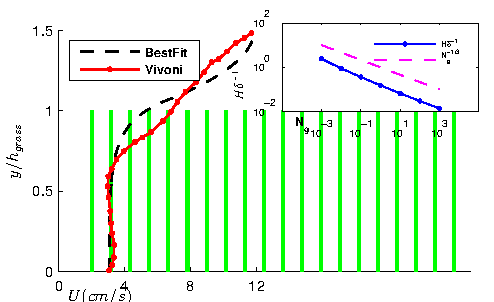
\includegraphics[scale=1]{Grass_Base_Vivoni_shear}
\caption{Basic flow profile (left )from the experiment and model and the model of canopy (bottom) along with variation of shear layer (inset) }
\label{fig:basicflow}
\end{figure}
\newline
Knowing the scale of shear layer we can systematically investigate its effect on flow instability
by varying grass number density $N_g$ and pressure gradient $\frac{dP}{dx}$. Considering small perturbations $u, v, p$ about the base profile $U$ and $P$
respectively, momentum and mass balance equation expanded in first order of perturbed variable yields
\begin{equation}
\begin{split}
\frac{\del u}{\del t}+U\frac{\del u}{\del x}+v\frac{\del U}{\del y} &= -\frac{1}{\rho}\frac{\del p}{\del x}+\frac{\mu}{\rho}\nabla^2u-2S(y) C_{N}dN_{g}Uu, \\
\frac{\del v}{\del  t}+ U\frac{\del v}{\del x} &= -\frac{1}{\rho}\frac{\del p}{\del y}+\frac{\mu}{\rho}\nabla^2v, \hspace{0.3cm} \nabla\cdot\bu=0.
 %\nabla\cdot \bu &= 0
\end{split}
\end{equation}
Momentum and mass balance equation can be non-dimensionlize using half channel height $H$, associated advection time H/$U_0$ and velocity $U_0$. We are left with three non-dimensional parameters in the model, viz. the Reynolds number $R= {\rho U_0 H}/{\mu}$, the drag parameter $\delta/H$, and the submergence ratio of the grass $h_g/H$. With these scaling along with the use of stream function $\psi$ with $u = \psi_{y}, v= -\psi_x$ to satisfy mass balance; 
% momentum and mass balance can be combined  into a single equation.
% \begin{equation}
% R \left[ (\del_t+\del_x U )\grad^2\psi - U_{yy}\psi_x \right] = \grad^4\psi-\frac{\del}{\del_y}\left({2}\frac{H^3}{\delta^3}S(y) U\psi_y\right).
% \end{equation}
Seeking wave solution in form of $\left(u,v,\psi \right)= \left(\hat u, \hat v, \hat\phi \right)e^{ikx+\sigma t}$,  we get modified Orr-Sommerfield equation. The eigenvalue $\sigma$ for a given $k$ provides growth rate and frequency associated with a perturbation of wavelength $2\pi/k$.
% \small
\begin{equation}
\begin{split}
\left(\sigma+ikU\right) \left(D^2-k^2\right)\phi &= \frac{1}{R_{e}}\left[D^2 -k^{2} \right]^2\phi +ikU_{yy}\phi \\
&-\frac{\del}{\del y}\left(\frac{2}{R_e}\frac{H^3}{\delta^3}S(y) U\phi_y\right)
\label{Orr-somerfield}
\end{split}
\end{equation}
% \normalsize

\begin{figure}[htb]
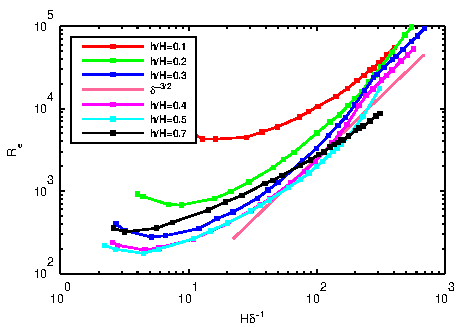
\includegraphics[]{Critical_Re_vs_delta}
\caption{Critical Reynolds number with flow for different grass height as a function of inverse shear thickness}
\label{Re_vs_delta}
\end{figure}
Solution of \eqref{Orr-somerfield} predicts a critical $R$ as function of grass number density, below which the flow is stable (Re($\sigma$)$<0$) and above which it is unstable (Re($\sigma$)$>0$),
as shown in Figure\ref{Re_vs_delta}. The solution also predicts a finite critical wavenumber $k$ corresponding to this threshold for instability shown in Figure \ref{K_vs_shear}. 
\shreyas{Needs language clean up from here on. Describe the most important observation. The details are to be explained in the longer paper.}
We observe that above a 
certain threshold $\delta$ the critical wavenumber is inversely proportional to $\delta$, similar to the one predicted by K-H theory based on the instability of free shear flow,
we identify this region as shear layer region. We also observe that once the $\delta$ is decreased below a critical value, there isn't any variation in the 
critical wavelength with the decrease of shear layer thickness and $\lambda_{critical} \sim (H-h_{grass})$, we identify this region as shear instability of unvegetated region.
The boundary of transition from instability of shear-layer near the tip of grass to the instability of unvegetated flow depends on the submergence ratio of grass. 
\begin{figure}[htb]
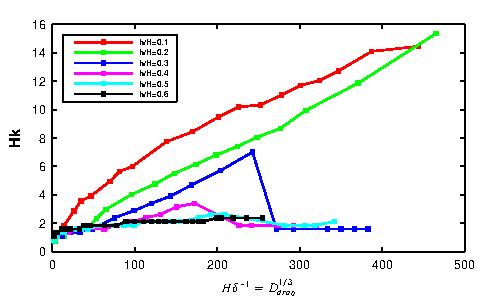
\includegraphics[]{K_vs_shear_width_noshear}
\caption{Critical Wavenumber for different grass height as function of shear layer thickness}
\label{K_vs_shear}
\end{figure}
\begin{figure*}
%\subfigure[]{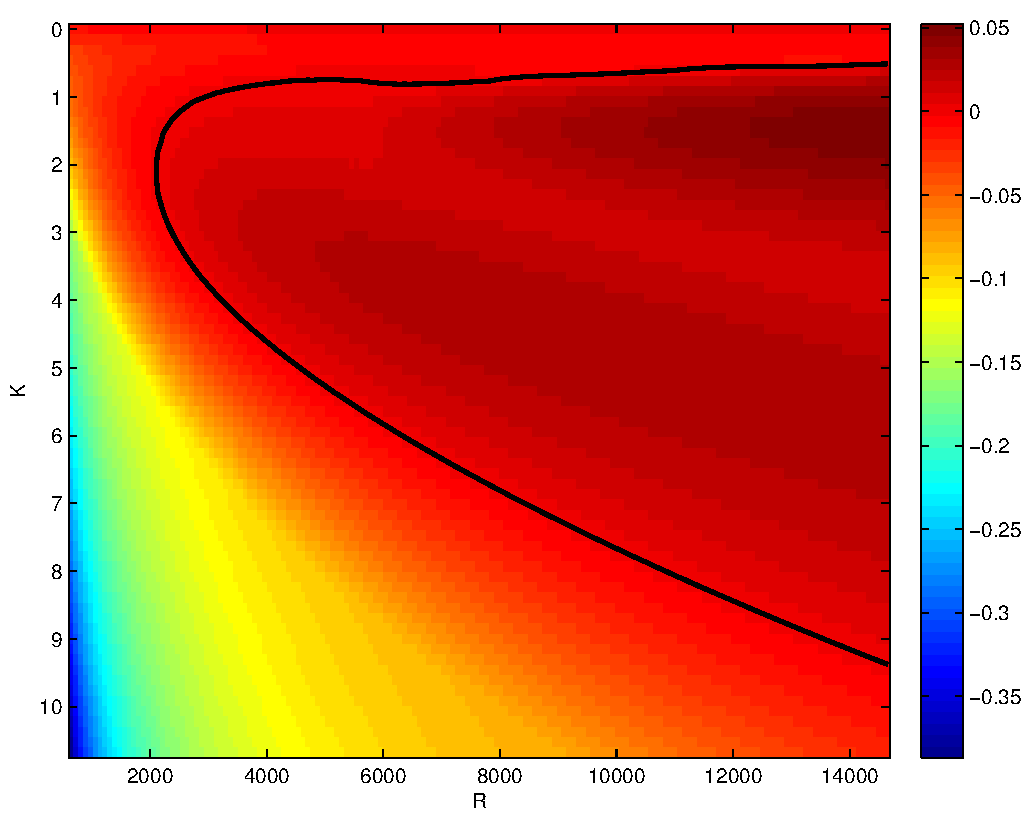
\includegraphics[scale = 0.24]{Set3_dens31_imgsc}}
%\subfigure[]{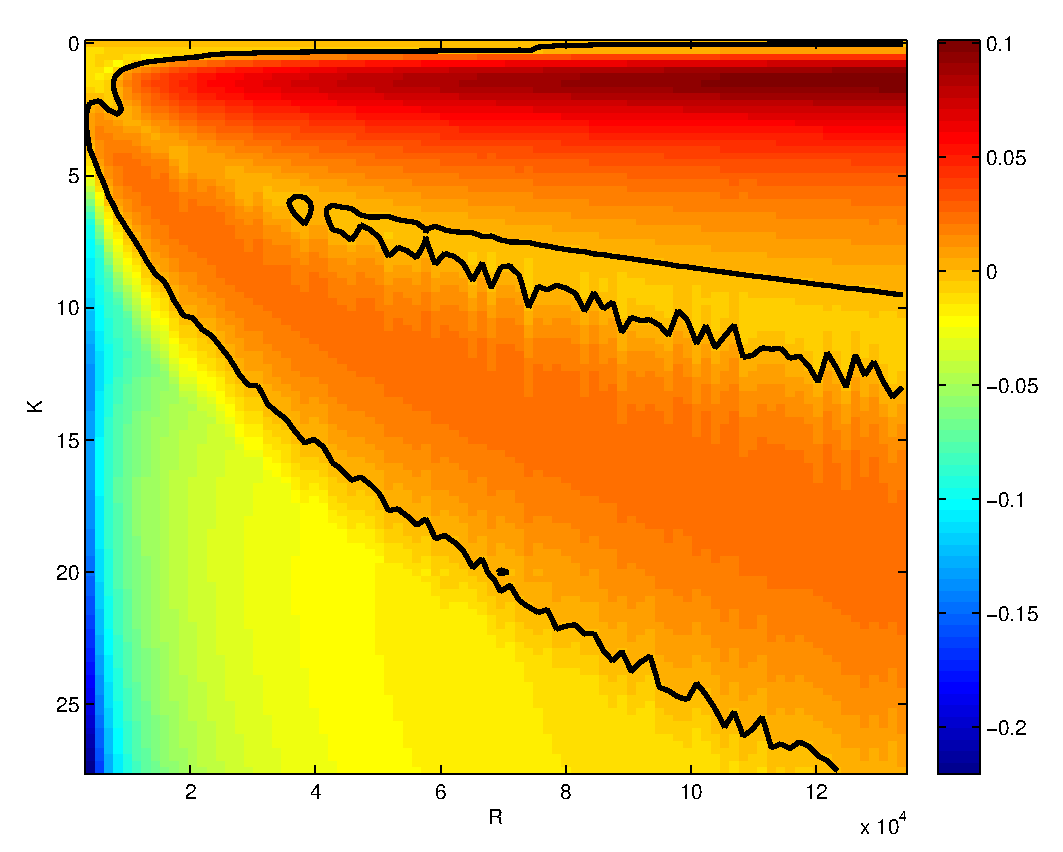
\includegraphics[scale = 0.24]{Set3_dens32_imgsc}}
%\subfigure[]{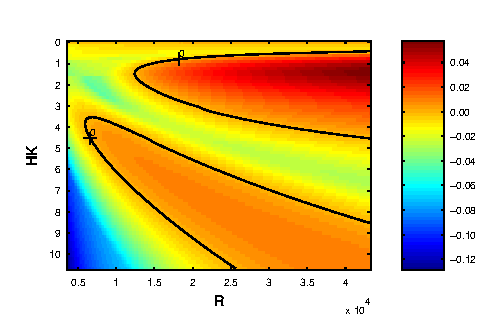
\includegraphics[scale = 0.24]{Set3_dens34_imgsc}}
%\subfigure[]{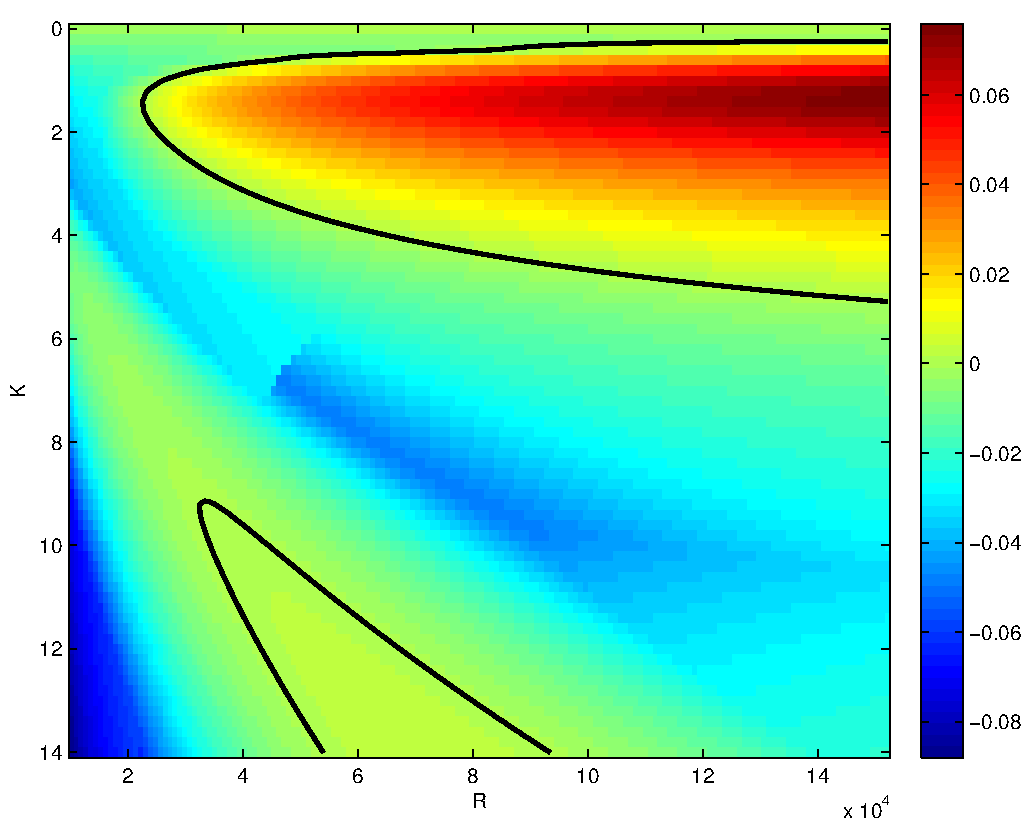
\includegraphics[scale = 0.24]{Set3_dens38_imgsc}}

\subfigure[]{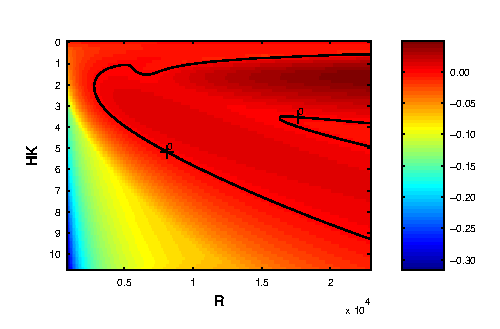
\includegraphics[scale = 0.55]{Set4_dens28_imgsc}}
\subfigure[]{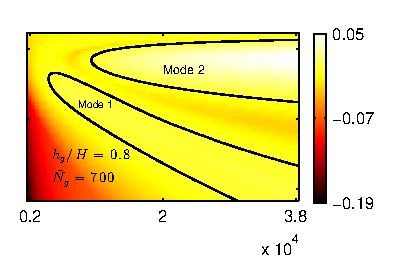
\includegraphics[scale = 0.55]{Set4_dens30_imgsc}}
\subfigure[]{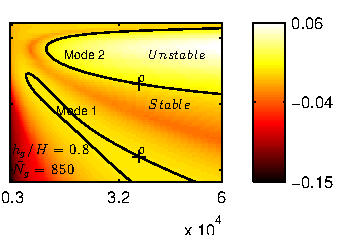
\includegraphics[scale = 0.55]{Set4_dens32_imgsc}}
\subfigure[]{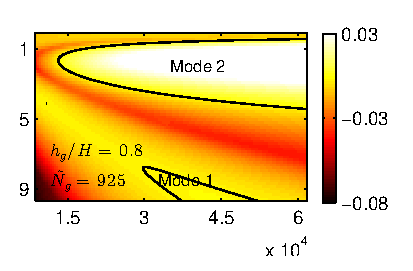
\includegraphics[scale = 0.55]{Set4_dens34_imgsc}}

\subfigure[]{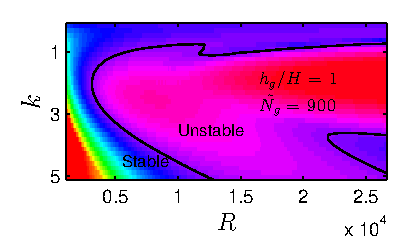
\includegraphics[scale = 0.55]{Set5_dens38_imgsc}}
\subfigure[]{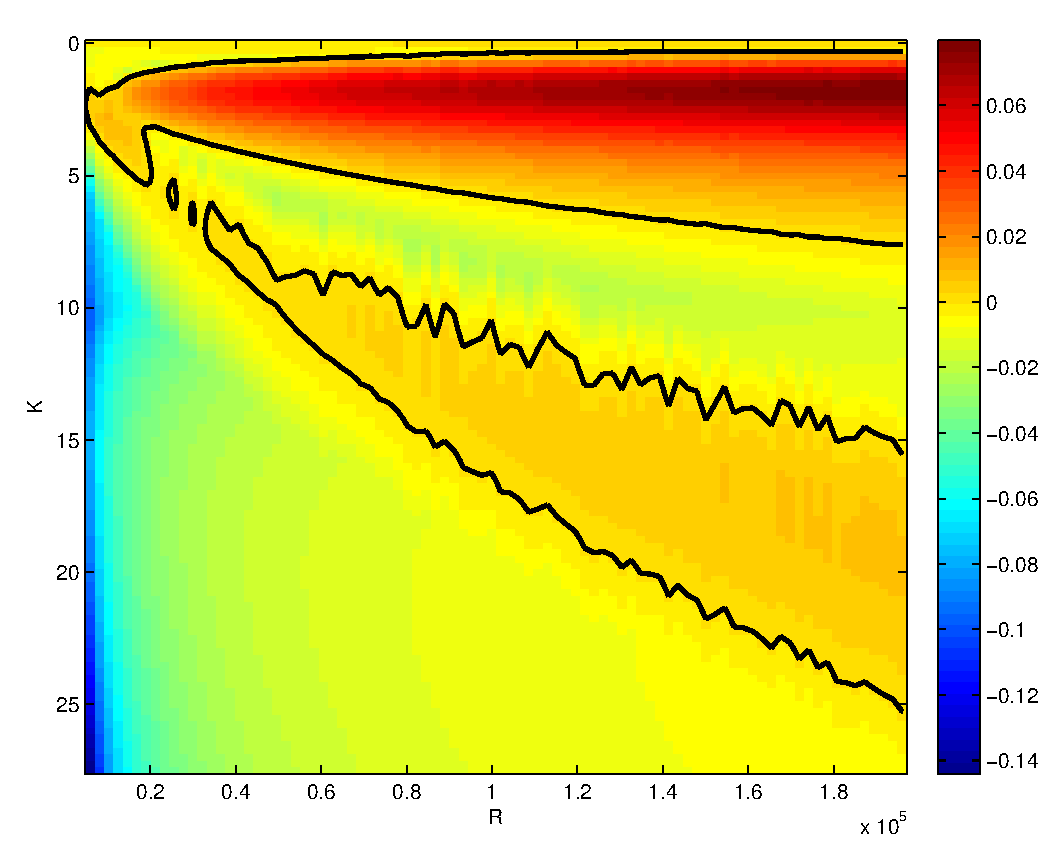
\includegraphics[scale = 0.55]{Set5_dens40_imgsc}}
\subfigure[]{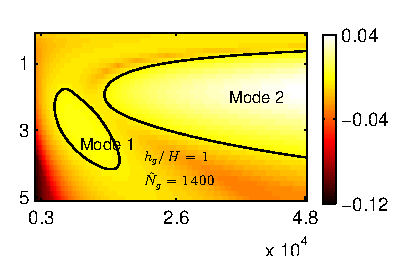
\includegraphics[scale = 0.55]{Set5_dens42_imgsc}}
\subfigure[]{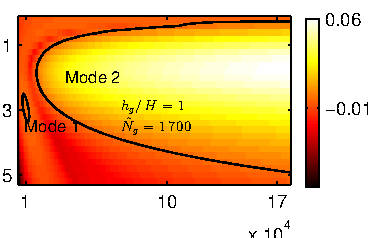
\includegraphics[scale = 0.55]{Set5_dens46_imgsc}}

\subfigure[]{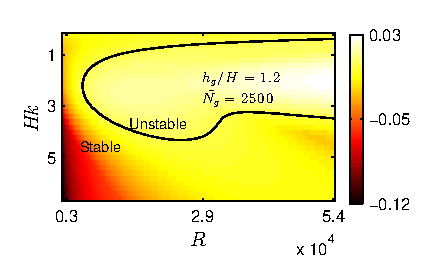
\includegraphics[scale = 0.55]{Set6_dens32_imgsc}}
\subfigure[]{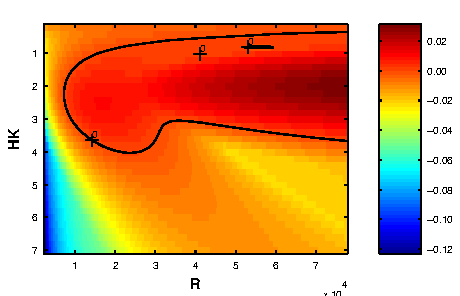
\includegraphics[scale = 0.55]{Set6_dens34_imgsc}}
\subfigure[]{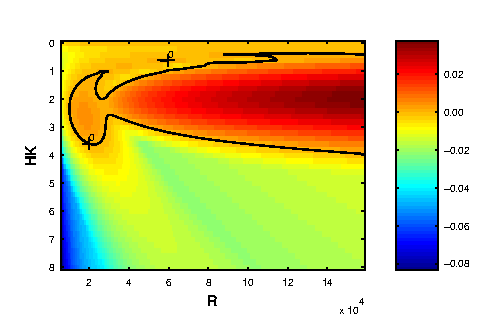
\includegraphics[scale = 0.55]{Set6_dens36_imgsc}}
\subfigure[]{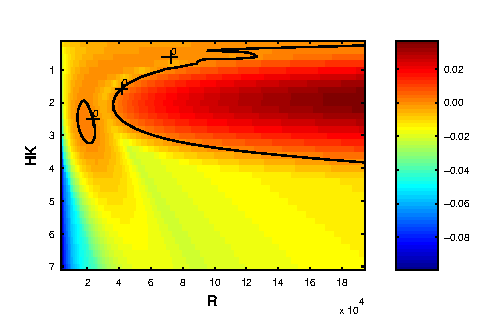
\includegraphics[scale = 0.55]{Set6_dens38_imgsc}}

\caption{$Re(\sigma)$ as function of wavenumber and Reynolds number for a given grass number density along with contour of zero growth rate ($Re(\sigma)$=0). The figures in each 
row corresponds to a particular grass height $h_{grass}/H = 0.8$ for (a-d), 1.0 for (e-h) and  1.2 for (i-l), these figures are arranged in order of increasing grass 
number density. At low grass number density both the modes are indistinguishable, but as $N_g$ increases the distinction between the two modes become clear. For $N_g$ below
a critical value, the K-H mode sets the onset of flow instability whereas above the critical $N_{g}$ onset of flow instability is dominated by shear instability of flow above the grass}
\label{K_Re_sigma_set3}
\end{figure*}
\newline 
The transition of dominant mode of flow instability from K-H mode to shear instability of flow above the grass can be further corroborated from Figure \ref{K_Re_sigma_set3}.
We observe that the two different modes of instability are indistinguishable at low grass density. The distinction becomes apparent with the increase in grass number density, where we 
can see that dominant mode of flow instability is 1st dominated by K-H mode before switching to shear instability of flow above the grass at relatively large grass density.  
%\newline
%The mechanism similar to Kelvin-Helmholtz instability is observed for a wide range of shear layer thickness for canopy with low submergence ratio $h/H\leq 0.4$.
%Canopy with low submergence ratio can also be related to the canopy in unbounded flow, such as terrestrial canopy with atmospheric flow with $h/H\sim 0$. 
%The linear variation of critical wavelength with the shear layer thickness for terrestrial canopy ($h/H \sim 0$) is consistent with the observed wavelength of honami 
%for terrestrial canopies.
%However, the deviation of critical wavelength from the prediction based on the instability of shear layer in region-1 and region-3 for a given submergence ratio shows the existence of 
%regimes where flow instability does not arise from mechanism similar to Kelvin-Helmholtz instability. The instability in region-1 is understood to be arising from instability of flow
%comprising flow in shear layer and flow above the canopies. The instability of flow comprising flow in shear layer and flow above the vegetation can be endorse by the linear 
%variation of the critical wavelength with the $H-h+b\delta$ in Figure \ref{Low_drag_k}, where $b\delta$ is the amount of perturbation of the flow into the vegetation.
\newline
%The constant value of critical wavelength for all the shear layer smaller than a critical value in region-3 suggest that the instability 
%in the region-3 is arising from the shear instability of flow above the canopy. 
%The existence of a regime dominated by shear instability of flow above grass is further corroborated 
%by the collapse of eigen-modes for different $\delta<\delta_{cr}$ ($\delta/H=0.0037,0.0034,0.0024$ in Figure\ref{Asymptotic_mode}) into a single profile as shown in 
%Figure \ref{Asymptotic_mode}, where $\delta_{cr}$ is the critical shear layer thickness
%below which instability of vegetated flow arise through the mechanism of shear instability of flow in unvegetated region rather than through the mechanism of Kelvin-Helmholtz type 
%instability of shear layer ($\delta/H=0.0052,0.0042$ in Figure \ref{Asymptotic_mode}). 
The regime of shear instability of flow above the 
grass further predicts that for large drag $R_e \sim (\frac{\delta}{H})^{-3/2}$, which can be understood by asymptotic analysis of \eqref{Orr-somerfield}.
Noting that for large drag, non-dimensional flow velocity $U \sim (\frac{\delta}{H})^{3/2}$ inside the grass and $R_{e} \gg 1$. So equation \eqref{Orr-somerfield}
can be simplified considerably both with in the grass and above the grass canopy. As $U_{yy}\sim 0$ inside the grass and $\frac{1}{R_e} \ll 1$,
the equation within the grass simplifies into
$\sigma\left(\phi_{yy}-k^2\phi\right) = -\frac{\del}{\del y}\left(\frac{2\phi_y}{\delta^{3/2}R_e}\right)$ while in the unvegetated region it simplifies into Rayleigh equation 
$ \left(\sigma+ikU\right) \left(D^2-k^2\right)\phi =  ikU_{yy}\phi$. From the balance of coefficients of $\phi_{yy}$ inside the grass we can easily estimate that asymptotically 
$R_e \sim (\frac{\delta}{H})^{-3/2}$.
\begin{figure}[]
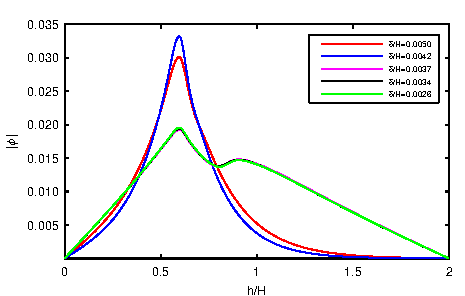
\includegraphics[]{Asymptotic_eig_set3.pdf}
\caption{plot of $|\phi|$ for different shear layer thickness in limit of small shear layer thickness}
\label{Asymptotic_mode}
\end{figure}
\begin{figure}[htb]
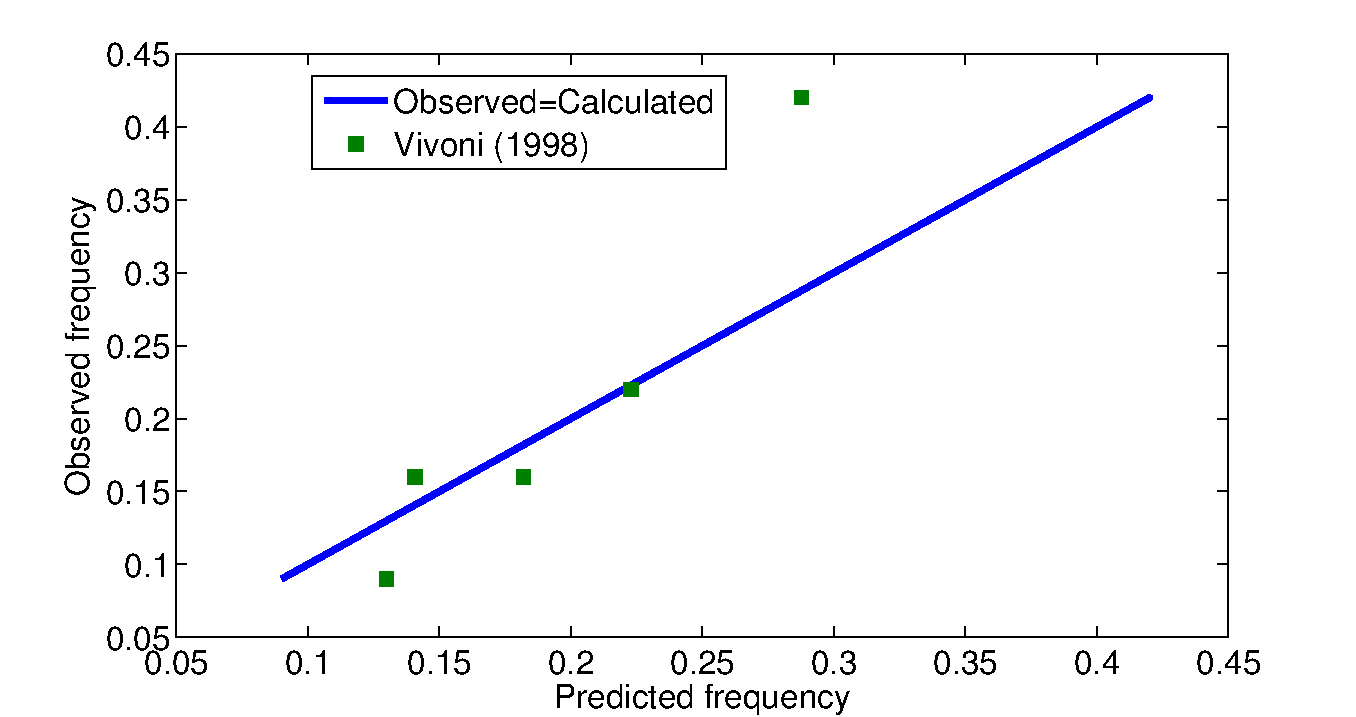
\includegraphics[scale=0.34]{Observed_vs_calculated}
\caption{Comparison between experimently oberved frequency and predicted frequency}
\label{Observed_calculated}
\end{figure}
\newline
Comparison of frequency associated with mode of highest growth predicted by model with that of experimental observations of frequencies in the lab scale experiments is shown in
Figure \ref{Observed_calculated}.
The observed frequencies in the lab scale are associated with the peaks in velocity spectra, frequency of monami and frequency of vortex passage. The agreement between the observed
frequency and the predicted frequency along with shear layer width suggest that monami is associated with the instability of flow comprising shear layer flow and flow above the canopy.
The deviation of predicted frequency from the observed one can be attributed to the various simplification we have made in our model. For real canopy the drag coefficients are known to
decrease from bottom to tip of the grass blades. The turbulent viscosity is also known to vary between the flow of unvegetated region and flow through the canopy. Although these variation
are not central to the mechanism leading to the instability of flow, we believe an improved analysis of flow with these variation in the model might lead to a better agreement between the
observed frequency and the predicted frequency.   
\newline
Numerical investigation of flow in presence of canopy reveal two distinct modes of flow instability which might lead to monami. The occurrence of these modes for flow instability in a 
canopy depends on its submergence ratio and shear layer thickness. Our analysis shows that flow in presence of grass become unstable not only through the mechanism similar to 
Kelvin-Helmholtz instability but also through shear instability of flow above the grass for small shear layer thickness and shear instability of flow comprising flow in shear layer 
with flow above the grass. Our analysis further predict a threshold criteria characterized by a Reynolds number above which flow become unstable. The predicted value of threshold
 Reynolds number is $O(100)$, which is 
close to the the Reynolds number corresponding to the observed value of threshold flow speed in the observation of Grizzle. Inclusion of variation of drag coefficient along the 
grass filament
might lead to better agreement between the observed and predicted frequency of monami. 



%\cite{Delangre06}\cite{Delangre04}\cite{Raupach96}\cite{Nepf99}
%\cite{Nepf02}\cite{Nepf04}\cite{Nepf08}\cite{Nepf08_2}\cite{Raupach11}\cite{Raupach94}
%\cite{Delangre06}
%\begin{figure}[htb]Q
%\subfigure{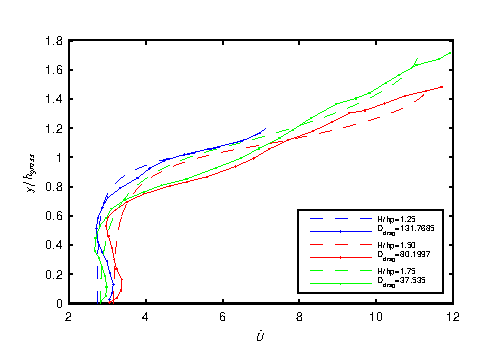
\includegraphics[]{Vivoni_Fig3_6_zero_shear_match}}
%\subfigure{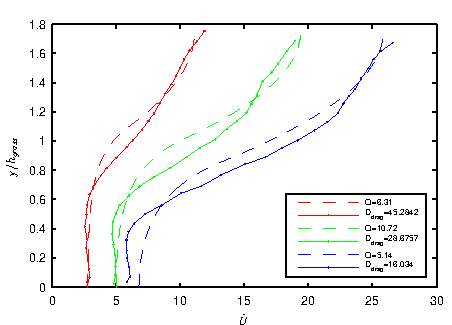
\includegraphics[]{Vivoni_Fig3_7_zero_shear_match}}
%\caption{Comparison between observed and calculated velocity profile}
%\end{figure}
%\begin{figure}[htb]
%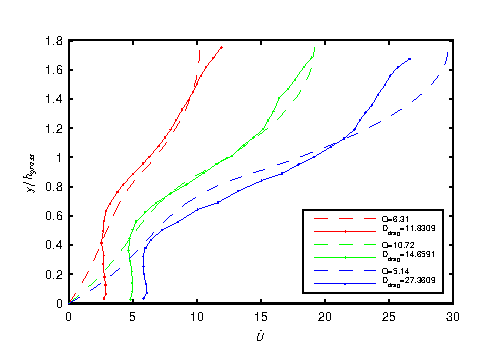
\includegraphics[]{Vivoni_Fig3_7_hb_14match}
%\caption{Comparison between observed and calculated velocity profile,hb=14}
%\end{figure}
%\begin{figure}[htb]
%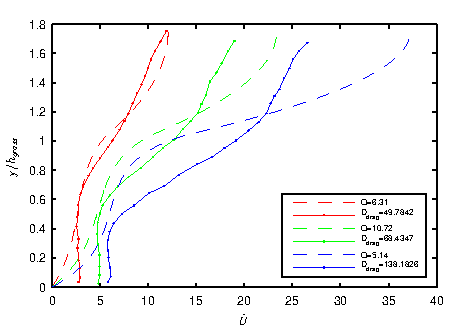
\includegraphics[]{Vivoni_Fig3_7_hb_17match}
%\caption{Comparison between observed and calculated velocity profile,hb=17}
%\end{figure}
\bibliography{Grass}{}
\bibliographystyle{plain}
%\nocite{*}
\end{document}
